\begin{center}
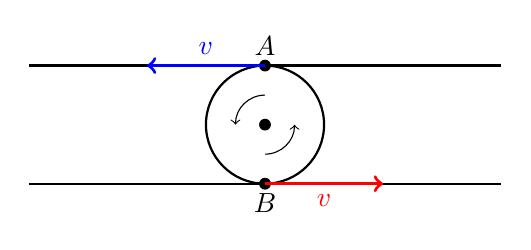
\begin{tikzpicture}[scale = 1.5]
			\draw[thick] (0, -0.5) -- (4, -0.5);
			\draw[thick] (2, -1) circle(0.5);
			\draw[thick] (0, -1.5) -- (4, -1.5);
			\fill (2, -0.5)node[above]{$A$} circle(0.05);
			\fill (2, -1.5)node[below]{$B$} circle(0.05);
			\fill (2, -1) circle(0.05);
			\draw[->, blue, very thick] (2, -0.5) -- (1, -0.5)node[midway, above]{$v$};
			\draw[->, red, very thick] (2, -1.5) -- (3, -1.5)node[midway, below]{$v$};
			\draw[->] (2, -1.25) arc (-90:0:0.25);
			\draw[->] (2, -0.75) arc (90:180:0.25);
\end{tikzpicture}
\end{center}
Рассмотрим, как движется шарик, если верхнюю пластину сдвигают в одном направлении. Шарик в общем случае может совершать поступательное движение и вращение. Можно перейти в систему отсчета, связанную с центром этого шарика. В ней центр шарика покоится, а все его движение связано с вращением вокруг центра. Тогда можно заметить, что скорости точек, в которых шарик касается пластин равны по величине и направлены противоположно друг другу. А так как проскальзывания нет, пластины движутся так же, как точки касания в данный момент времени.
\begin{center}
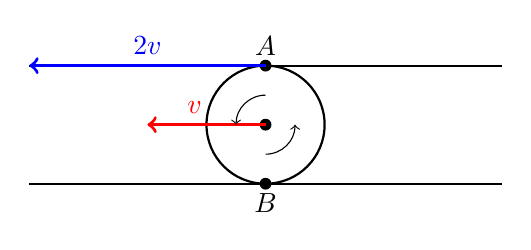
\begin{tikzpicture}[scale = 1.5]
			\draw[thick] (0, -0.5) -- (4, -0.5);
			\draw[thick] (2, -1) circle(0.5);
			\draw[thick] (0, -1.5) -- (4, -1.5);
			\fill (2, -0.5)node[above]{$A$} circle(0.05);
			\fill (2, -1.5)node[below]{$B$} circle(0.05);
			\fill (2, -1) circle(0.05);
			\draw[->, blue, very thick] (2, -0.5) -- (0, -0.5)node[midway, above]{$2v$};
			\draw[->, red, very thick] (2, -1) -- (1, -1)node[pos=0.6, above]{$v$};
			\draw[->] (2, -1.25) arc (-90:0:0.25);
			\draw[->] (2, -0.75) arc (90:180:0.25);
\end{tikzpicture}
\end{center}
Тогда вернемся в систему отсчета, в которой нижняя пластина покоится. В ней нижняя точка шарика покоится, а центр шарика движется сонаправлено с верхней пластиной со скоростью $v$. Верхняя пластина движется в этот момент со скоростью $2v$. Значит можно сделать вывод о том, что скорость центра шарика всегда вдвое меньше скорости пластины, а значит вдвое меньше и все перемещения. Траектория шарика, в таком случае, будет иметь такую же форму, как траектория центра пластины, но длины всех линий будут уменьшены в два раза. Тогда с соблюдением масштаба она будет выглядеть так
\begin{center}
	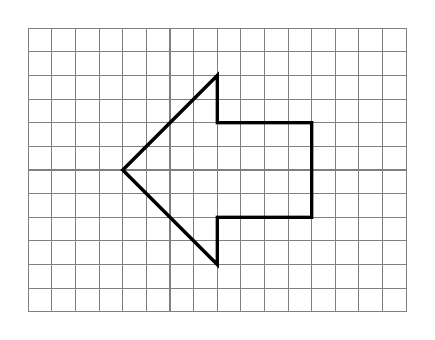
\begin{tikzpicture}[scale = 1.2]
		\draw[step=0.25,gray,thin] (0, 0) grid (4,3);
		\draw[very thick] (1, 1.5) -- (2, 0.5) -- (2, 1) -- (3, 1) -- (3, 2) -- (2, 2) -- (2, 2.5) -- cycle;
	\end{tikzpicture} \ \ \ \
	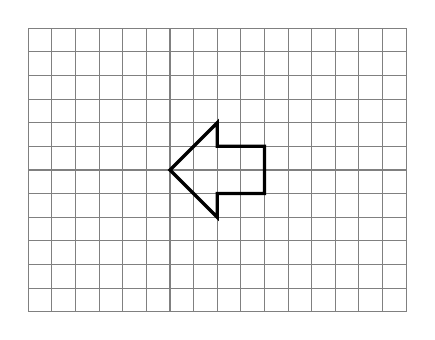
\begin{tikzpicture}[scale = 1.2]
		\draw[step=0.25,gray,thin] (0, 0) grid (4,3);
		\draw[very thick] (1.5, 1.5) -- (2, 1) -- (2, 1.25) -- (2.5, 1.25) -- (2.5, 1.75) -- (2, 1.75) -- (2, 2) -- cycle;
	\end{tikzpicture}
\end{center}

\ifgrade
\begin{grade-env}
	\grade{2}{Утверждение о том, что смещение шарика вдвое меньше смещения пластины.}
	\grade{2}{Верный ответ в виде рисунка с соблюдением масштаба.}
\end{grade-env}
\fi